\documentclass[twoside,reqno]{article}

\usepackage[utf8]{inputenc}
\usepackage{graphicx}
\usepackage{float}
\usepackage{subfigure}
\usepackage[version=4]{mhchem}
\usepackage{hyperref}
\usepackage{booktabs}
\usepackage{algpseudocode}
\usepackage{algorithm}

\usepackage{setspace}
% \usepackage[showframe]{geometry}
\usepackage[]{geometry}
\newcommand{\ch}[1]{\MakeUppercase{\ce{#1}}}  % version 1
\newcommand{\multiref}[2]{\autoref{#1}-\ref{#2}} % from - to
\newcommand{\qfig}[4]{\begin{figure}[H]\centering\includegraphics[width=#4]{#1}\caption{#3}\label{#2}\end{figure}\newpage}
% location,label,caption,width

\algnewcommand\algorithmicforeach{\textbf{for each}}
 \algdef{S}[FOR]{ForEach}[1]{\algorithmicforeach\ #1\ \algorithmicdo}
\algnewcommand\algorithmicforeach{\textbf{for each}}
\algdef{S}[FOR]{ForEach}[1]{\algorithmicforeach\ #1\ :}

\def\blankpage{%
      \clearpage%
      \thispagestyle{empty}%
      \addtocounter{page}{-1}%
      \null%
      \clearpage}

%%%%%%

\title{Model diagnostics and sensitivity methods through graph-based network analysis.}
\author{Dan Ellis }
\date{March 2019}

\begin{document}
% \newgeometry{oneside}
\maketitle

\restoregeometry
\blankpage
\doublespacing
% \onehalfspacing
\newpage
\section*{Results Chapter II}
\tableofcontents
\newpage

\raggedbottom %group writing to top of page!
\section{Introduction}
Comprehensive understanding of the chemical system underpinning reactions in the atmosphere is paramount when it comes to predicting changes in both air quality and climate. Our knowledge of the chemistry is often derived using chemical understanding, pre-existing theory and experimental measurements [REF IDEAS?]. Unification of this knowledge in the from of first order differential equations, describing all possible reactions within a system, form a mechanism.




% These combination of these results to form a mechanism \footnote{A series of first order differential equations representing the existing pathways and reaction rates between species} and in turn the foundation of all models.

One prominent issue that exists in both mechanism development and model analysis is measuring how changes are perturbed within the system. Real world networks often exhibit `small-world phenomena` [SEVERAL REF power law?], with chemical networks showing no exception. Analysis of the full Master Chemical Mechanism\footnote{Version 3.3.1} (MCM) show it takes on average XXX reactions to travel from a species to any other non-emitted species. It the complex and entwined nature of reactions within the mechanism that make the tracking of changes and errors within a mechanism a highly difficult problem.


\begin{figure}[H]
    \centering
    %  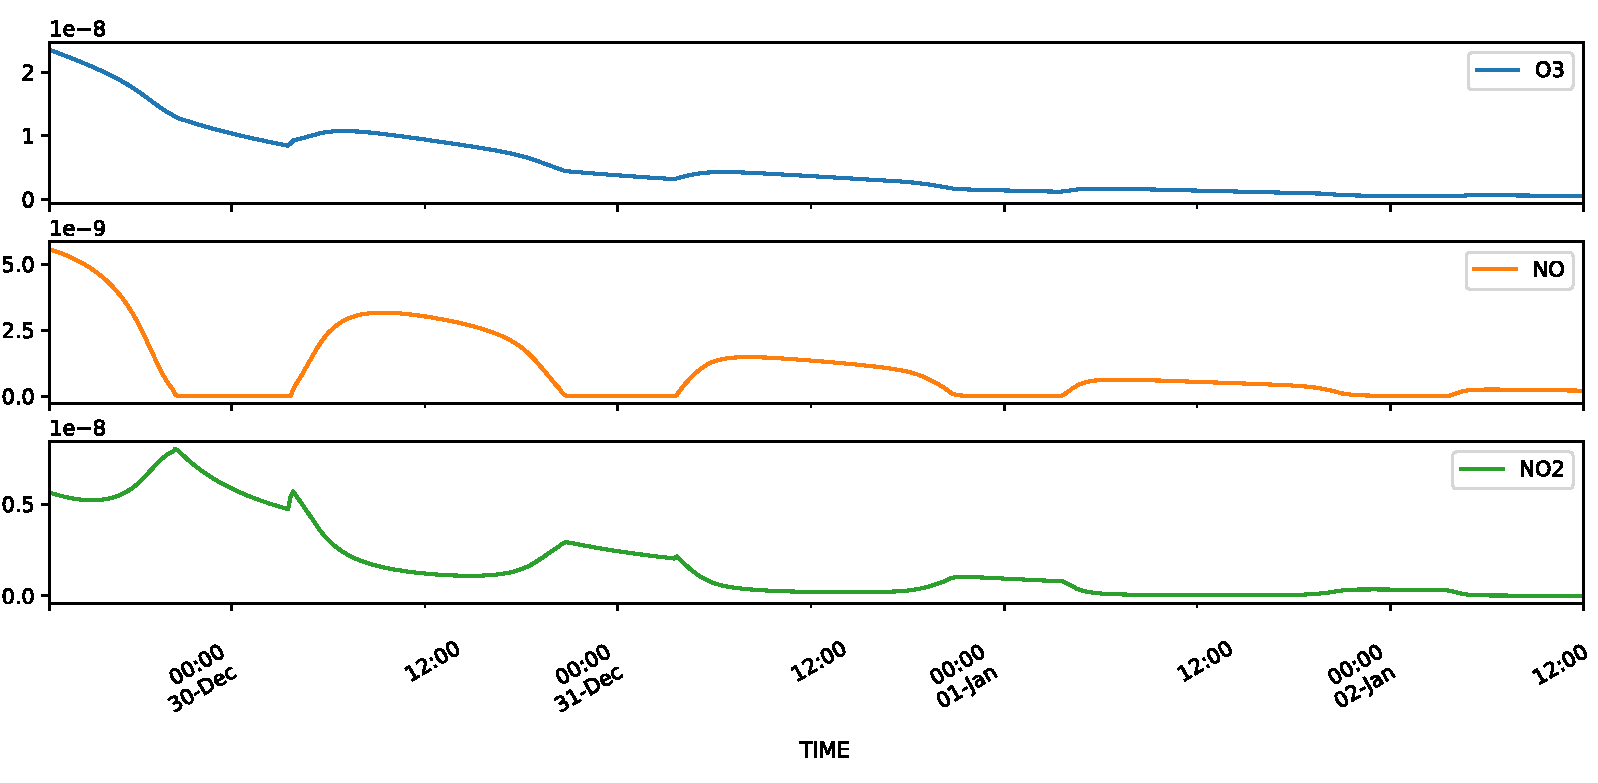
\includegraphics{figures/ch2concentration.pdf}
    \caption{An example plot of the whole MCM with each node coloured how easy it is to be reached by every other node. }
    \label{fig:smallworld}
\end{figure}

\subsection{The Model}

The following section will descibe...
- from the MCM will be used. This is propagated forward up until steady state, using the Dynamically Simple Model of Chemical Complexity (DSMACC)[REF 1,2] and then run forwards in time for one day. A figures

\section{Existing Methods}

Historically there have been three main methods for model interpretation: concentration, flux and Jacobian analysis. The simplest of these involves looking at how a species concentration changes over time.


\subsection{Concentration time series}

The concentration of a species is a description of its abundance within the atmosphere. As models are run forwards in time, bonds are made and broken, changing the chemical composition of reactants to products. This shifts concentration from the initial conditions towards their ultimate destination.

Examination of how a species concentration changes over time enables us to determine influential factors and traits of the system -for example  \autoref{fig:concentration} suggests an inverse relationship between \ch{NO2} and \ch{NO} relating to time of day.

% policy focused prediction.

\qfig{figures/ch2concentration.pdf}{fig:concentration}{Concentration time series: The classic method for identifying changes in a model. This multi-plot shows the changes in concentration profiles for all initialised species following an initial spin-up to steady state. }{.8\textwidth}

\subsection{Rate of Production and Loss}

Concentration analysis allows us to juxtapose final or maximum results for varying model / scenario simulations, however they do little to quantify the extent of the change.

In policy focused simulations, once a species of interest has been identified, we then become interested in determining which reaction pathways are responsible for its production and loss. Rate of Production \footnote{and loss} Analysis (ROPA) provides a method for isolating the cause of the change within a species concentration.

Taking \autoref{fig:ropa_day} as an example, the ROPA plot allows us to rank the most influential reactions in the production of \ch{CH3CO3}. In complex multi-body reactions isolating the exact cause of concentration change may prove difficult. Cyclic reactions, such as \ch{PAN} $\longrightarrow$ \ch{CH3CO3} + \ch{NO2} and \ch{CH3CO3} + \ch{NO2} $\longrightarrow$ \ch{PAN}, suggest a high importance to the production and loss of \ch{CH3CO3}. However with both reactions of similar magnitude and opposing directions the net effect is only marginal. To account for this we can calculate the individual contributrion of one species on another using the Jacobian method.

\qfig{figures/ROPA_CH3CO3.pdf}{fig:ropa_day}{Rate of production and loss analysis plot for \ch{ch3co3} exhibiting a net production (daytime)}{\textwidth}



\subsection{Using the Jacobian Matrix}

In a model the Jacobian is a square matrix of partial derivatives. This is used to predict the future state for all species within a mechanism and is calculated by taking the gradient for each reaction, in turn determining the individual (partial) contribution of each species. These partial equations are then summed to determine the total contribution of species $i$ on $j$ and used to populate the $J_{i,j}$th element of the Jacobian matrix. Values of the jacobian tell us the extent of how a 1\% change in species $i$ affects species $j$.

Jacobian analysis is the most effective way to establish which species have the greatest influence on the system.


important species and forms the foundation of connectivity based reduction methods [ref connectivity method and em connectivity method], where redundant species are removed from a mechanism. Applying this to determine the contribution of species for \ch{CH3CO3} produces [TABLE REF]. This shows a much clearer image of the contributing species than \autoref{fig:ropa_day}, and that although fifth most reactive equation in the ROPA analysis, the the decomposition of \ch{CH3COCH2O} has the greatest influence on \ch{CH3CO3}.\\


% p = w.apply(lambda x: ('%.1e'%x).replace('e','$\times 10^{')+'}$ %')
% print p.to_latex().replace('textbackslash ','').replace('\$','$').replace(r'textasciicircum','^').replace('\}','}').replace('\{','{').replace('\^ ','^')
\begin{table}[H]
\centering
\begin{tabular}{cc}
\toprule
Species Name & Net-contribution (\%) \\
\midrule
\ch{CH3COCH2O} &  9.9$\times 10^{-01}$  \\
\ch{CHCO2}   &  2.7$\times 10^{-06}$  \\
\ch{NO2}       &  1.5$\times 10^{-06}$  \\
PAN       &  1.2$\times 10^{-06}$  \\
MGLYOX    &  1.4$\times 10^{-10}$  \\
HYPERACET &  4.4$\times 10^{-12}$  \\
ACETOL    &  4.4$\times 10^{-12}$  \\
\ch{CH3COCH3}  &  1.3$\times 10^{-12}$  \\
\ch{CH3CHO}    &  2.0$\times 10^{-15}$  \\
OH        &  6.7$\times 10^{-28}$  \\
\ch{CH3CO3H}   &  3.3$\times 10^{-30}$  \\
\ch{CH3CO2H}   &  8.6$\times 10^{-31}$  \\
\ch{O3}   &  6.5$\times 10^{-31}$  \\
\ch{NO3}       &  6.4$\times 10^{-32}$  \\
\bottomrule
\end{tabular}

\caption{Jacobian analysis showing the $log_{10}$ - [0,1] normalised net-contribution a species to \ch{CH3CO3}.  }
\end{table}

\subsubsection{Summary of current methods}
If quantifying change is needed for policy or scenarios based simulations, the use of concentration profiles is more than adequate to obtain such results. If further information on the reactions causing such a change is needed, we may look at the flux (rate of change of concentration) from each reaction contributing to it. Finally if we wish to know how changing a concentration will effect one, or many, species, we must examine the effect of all contributing components for each production and loss flux. This may be done by comparing values present in the Jacobian matrix.



\section{Graph based methods}
Graphs may be considered as abstract representations of real world networks. These often consist of a series of nodes (species) connected by a common property (the influence of one node on another). The Jacobean matrix is a descriptor for how the transformation of the chemical system from one latent space to anther. Similarities between this and a graph adjacency matrix make the conversion between them almost trivial by taking the $log_{10}$ and normalising between 1 and 0.

Having generated a representation of the chemical network within a simulation it is now possible to apply a range of network tools to

and are often represented in matrix form. Much like atmospheric Chemistry, one of the primary purposes of network analysis is the identification of `important' nodes within the system, \cite{abstract-realworld}. In converting the Jacobian into a adjacency, or relationship, matrix it is possible to generate a graph representing the chemical network of our simulation.


Centrality metrics,,, BACKGROUND REF USAGE \href{http://moreno.ss.uci.edu/91.pdf}{http://moreno.ss.uci.edu/91.pdf} <- a comprehensive introduction on the histtory  \cite{dev-social-analysis} \\



Within small networks $~ 30$ nodes, visual interpretation of both nodes and reactions of interest may be possible. However with large automatically generated mechanisms of $> 5000?$ species we are forced to rely on computational mathematics, in the form of centrality metrics.

All centrality metrics listed below may be perfomred by the IGRAP ref or NetworkX packages in python, and many others elsewhere.


\subsection{Unweighted Directed Analysis}

Degree, Hubs and Authorities are weight in dependant metrics. This means that they do not require a simulation to be run in order to produce the required result. It is possible to generate the required dyadic or binary adjacency matrix, \autoref{binary}, directly from the mechanism file.

\begin{equation}
    A_{ x,y}=
    \begin{cases}
      1, & \text{if           $x\xrightarrow{prod.}y$}\\
      0, & \text{else}
    \end{cases}\label{binary}
\end{equation}

\subsubsection{Degree}
Degree centrality \cite{degreefreeman}, provides a description of the total number of links incident upon a node. In the real world this has applications ranging from locating popular topics in a social media project to reducing auction fraud \cite{degreetwitter,degreefreeman}.


Within the chemical system, nodes with a high degree undergo reactions with many other species. This by proxy suggests potential difficulty in isolating the source of any changes within their concentration, or attempting to remove them when reducing a mechanism.

For a directed network, reaction links may be split into production and loss reactions. This allows us to determine the nature of a node due to the number of reactions it yields. For instance a node with high in-degree is a species produced by many others - for instance \ch{co}. Alternatively large reactive hydrocarbons with many outwards reactions will have a high out-degree.

\subsubsection{Hypertext Induced Topic Search (HITS)}
HITS \cite{hits,hitsvspagerank} is an eigen-vector algorithm originally used to rank and classify web pages \cite{hitsweb}into two categories: Hubs and Authorities.

For a chemical mechanism, Hubs are species with many in-going links, and are predominantly produced by other reactions. Authorities on the other hand tend to be reactants, which produce many other species. In general these tend towards larger hydrocarbons, with long lifetimes, that are difficult to make.

\autoref{fig:degree} shows that species, all with lots of reactions (a high degree) may have very different roles within a network. Since the MCM does not explicitly define carbon dioxide, much of the chemistry flows towards \ch{CO}. This by the nature of reactions makes carbon monoxide a hub. Alternatively XXXXXXXX acts as a YYYYY and produces many other species, and is therefore classified as a strong authority. Finally Formaldehyde contains both many production and loss links. It is for this reason both a hub and an authority, making it both an important precursor and product to many species within the network.



\subsection{Weighted Degree}
Similar to the unweighted degree, we are able to scale node rankings with the strength associated with each reaction. In weighting the edges with respect to the influence between nodes, we are able to discern nodes with lots of reactions from nodes with lots of `fast' reactions, \autoref{fig:linkscoloured}. In subtracting loss reaction weights from production weights we are able to calculate the net flux\footnote{$\dot{v}$ if you are using KPP {REF KPP}} flowing through a node. \autoref{fig:weighted} adds an additional layer of information on how the chemistry is propagated within the model at that point in time. This allows us to better rank a nodes importance.

\qfig{newfigs/ch2_hubs_auth.pdf}{fig:degree}{
A bivariate cloropleth depicting hubs, authorities and degree (node size). It is seen that our primary hydrocarbons are both small in size (few reactions) and hubs of the chemistry (they produce other species rather than being produced). }{\textwidth}

\qfig{newfigs/ch2_weighted.pdf}{fig:linkscoloured}{A representation on the which links hold the greatest influence. Pink are the highest, and Blue are the lowest. Node size represents the net flow going through a node (the weighted degree). }{\textwidth}

\qfig{newfigs/ch2_weighted_degree.pdf}{fig:weighted}{A representation on the which links hold the greatest influence. Pink are the highest, and Blue are the lowest.}{\textwidth}




\subsection{Shortest Path}
We are able calculate the contributions to a single node from every other
node by summing the weights of the path taken to get to it. Unlike the Jacobian based connectivity method, this not only shows the direct contributions to a species, but also the indirect contributions. In taking the shortest path between two nodes, we eliminate the need for recursive iteration required by the connectivity method, allowing for a simpler process, coupled with a more intuitive understanding of the hierarchical contributions in the creation of a species.



One compound often explored is the formation of formaldehyde (\ch{hcho}), least because of its cancerogenic nature {REF}, but more its role as a precursor to many other carbon compounds [ref mcm and btetweeness graph?].\\

\subsection{The hierarchical subgraph of influence.}

Application of this method exposes the hierarchical nature of species formation which is seen in many real-world systems [SMALL WORLD / POWER law REF] \autoref{fig:treeform} shows the different route various species may take to influence the formation of formaldehyde.

As a better representation of weighted hierarchical data, it is possible to use a D tree-map \cite{treemap}, an improvement on the previously used Mosaic plot \cite{mosaic}. The nested nature of \autoref{fig:treemap} allows extended insights, such as \ch{ch3o2} acting more as a proxy for \ch{ch3co2h} which in turn is heavily influenced by \ch{ch3co3} rather than presenting a large influence in itself. Viewing the chemistry in this way not only places an emphasis on the complexity of chemistry in the atmopsphere, but also the
indirect effects one species may have on the formation of another.

\qfig{newfigs/ch2_distance.pdf}{fig:distance}{An edge bundled  force directed layout with variable link widths to visualise the shortest paths to \ch{HCHO} from every other node. }{\textwidth}


\qfig{figures/treeformation.pdf}{fig:treeform}{     WRONG ! A radial tree representation showing the route of influence for each species in the network to formaldehyde.}{\textwidth}


\qfig{figures/treemap.pdf}{fig:treemap}{WRONG ! A treemap nested nature of chemical influence upon \ch{hcho} and each species contribution.}{\textwidth}


\subsubsection{Closness Centrality}
Closeness centrality is an continuation of the shortest path algorithm, extended such that it ranks all nodes within a network on their ability to convey information to everyone else. A nodes closeness is calculated by taking the reciprocal of the sum of dijkstra paths\footnote{the shortest available path} to every other species \cite{closeness-book,closeness}. Historical applications include intelligence gathering in terrorist networks, estimating arrival time in telecommunications packages and calculating the importance of words in key-phrase extraction \cite{terror,examples_centrality,phrase}.

A chemical species with a high closeness centrality holds a higher global impact on the network, should its concentration change.



\subsubsection{Betweenness}
In social networks it is often important not only to know who has the greatest reach (closeness centrality), but also where the bottleneck or `broker' positions are.
The betweennes of each node represents the number of number of geodeisic (shortest) paths that pass through it for the whole network. Any conditions where there are multiple possible paths are handled by the denominator \cite{betweenness,between,betweenfast,examples_centrality}.

For a chemical network, species which act as either enables or limits the flow of information to sections of a network. If a species is on the shortest path for a set of nodes, it can me though of as `pivotal' \cite{neoj4}. Should a pivotal node be removed, we either a longer `shortest' path will be located, hindering the network, or even isolating the two groups connected to that node. Pivotal species could be thought of as important due to their ability to throttle the production or loss of other species within the network.

\subsubsection{Comparing Closeness with Betweeness}
 Some description of \autoref{fig:closebet} here.


\qfig{newfigs/ch2_between_close.pdf}{fig:closebet}{A representation on the which links hold the greatest influence. Pink are the highest, and Blue are the lowest.}{\textwidth}


\subsection{Spectral methods for matrix analysis.}
Spectral raking is a field of mathematics which applies the theory of linear maps, such as eigen-vectors and values, to stochiometric data in matrix form. Although spectral methods have been around since the 50's \cite{seeley}, they were only made popular after Larry Page's creation of the google page-rank algorithm \cite{google}. Spectral methods, such as HITS algorithm (already discussed), use a graphs matrix representation to calculate node importance. Of the many methods that exist, these can often be broken down into four basic categories, \cite{spectral}.

\begin{table}[H]
\begin{tabular}{l||cc}
\hline
 &No Normalisation  & Row Normalisation \\
 \hline \hline

No Damping &
 \shortstack{Eigenvector \cite{eigen,eigen2} \\ \:}
 & \shortstack{ Markov Chain Steady \\ State \cite{seeley} \\ \:} \\

Damping &
 \shortstack{Katz \cite{katz}\\ \:}
 & \shortstack{Total Effect Centrality, \\ PageRank \cite{google}} \\
 \hline
\end{tabular}
\end{table}


Here damping terms represent the probability of moving to new random starting position, allowing for the user to `randomly select a new webpage' or leave a isolated cluster. Normalisation of the matrix, does not affect the node ranking, but merely adjusts the numerical output of the algorithm. It is for this reason that its overall practicality may be debated \cite{spectral}. Since page rank is the most common of these methods and allows for a tune-able degree of randomness within network propagation, this shall be discussed in more detail .


\subsection{Page Rank}


Page rank is the best known of all centrality algorithms \cite{neoj4}. As with all eigenvector methods, it measures the transitive influence in nodes, taking the effect of neighbours, and by proxy, their neighbours into account. In the context of web pages or citations, a link from a highly ranked, or credible, source holds more weight than one one from someone less credible. \\


History of page rank, app web pages citation counts. biophysics , etc, etc,..

\subsubsection{The Google Matrix}
In order to solve for page rank, one must first construct the google matrix. Once this has been done, iterations of the power method can be applied until convergence is reached. \\

Building the google matrix begins by turning our graph adjacency matrix $A_{i,j}$ into a Markov matrix $M_{i.j}$. The simplest way is to take our dyadic link map \autoref{binary}, and divide each column $j$ by the sum of the total outgoing links of node $j$, Algorithm \ref{eqn:markov}. Dangling nodes are species with no outgoing links. In chemical mechanisms these are generally removed, but could represents sinks within a system. In the case of dangling nodes, either a personalised list of values or a constant value, $1/n$, replaces the zero columns\footnote{Where $n$ is the number of nodes}.  This construction results in a normalised\footnote{ \: $\Sigma_{i=1,n} M(i,j) = $ unity} matrix of markov chains representing the fractional production for node $j$ from all other nodes. \\

\begin{algorithm} \caption{Adjacency to Markov matrix.}
\begin{algorithmic}[1]
\State Obtain graph adjacency matrix, $A_{i,j}$.
\Repeat
\ForEach {$ j \in \mathcal $columns }
\State $M($:$,j) \gets A($:$,j) / \Sigma_{i=1,n} A(j,i)$
\EndFor
\Until {$\Sigma_{i=1,n} M(i,j) = 1$}

\end{algorithmic}\label{eqn:markov}
\end{algorithm}



The google matrix can now be defined using \autoref{eqn:google}. Cyclic reactions and nodes that only point towards each other within a group can `trap' the user, increasing their ranks. A damping factor, $\beta$, can be used to reduce this though selecting a probability that a used follows an existing link, typically $\beta = 0.85$, and a probability that they randomly select another page\footnote{Also known as teleporation.}, $(1-\beta)$. The value of $\beta$ will vary with application - a study in the application to biological data found an optimum value of $\beta = 0.694$ using Bayesian analysis \cite{biopr}, however in most cases the typical value will suffice.


\begin{center}
\begin{equation}
     G_{i,j} = \beta M + \cfrac{1 - \beta}{n}
 %\vec{dsfds}
 \label{eqn:google}
\end{equation}
\begin{tabular}{ccl}
$\beta$&-&\textit{Probability the user follows a link} \\
 $(1 - \beta)$&-&\textit{Probability the user does not follow a link (teleportation)} \\
$n$&-&\textit{Number of items / species}\\
$M$&-&\textit{Normalised markov matrix}
\end{tabular}
\end{center}


\subsubsection{Solving the algebra}

Once defined, the google matrix can be solved by propagating a ones vector, $r$ of length $n$, where $n$ is the number of species using Algorithm \ref{eqn:forwards}. This is repeated until a pre-defined tolerance, $\epsilon$ is reached. For best results this can be set to the programs precision.

\begin{algorithm} \caption{Solving the google matrix linear algebra}
\begin{algorithmic}[1]
\State {Define value vectors $\Bar{r}_t$ and $\Bar{r}_{t+1}$:}
\State  $\Bar{r}_t \:\:= [1_1, 1_2, ... , 1_n]$, $\Bar{r}_{t+1} = [0_1, 0_2, ... , 0_n]$
\State
\While {$||\Bar{r}_{t+1} - \Bar{r}_t|| > \epsilon$}
\State $\Bar{r}_{t+1} \gets M . \Bar{r}_t$
\State $\Bar{r}_t = \Bar{r}_{t+1}$
\EndWhile
\end{algorithmic}\label{eqn:forwards}
\end{algorithm}

For smaller systems it is possible to use lapack \cite{lapack}, linear algebra solvers such as those used by numpy \cite{numpy}. However if a network is large, computing an $n \times n $ matrix may be very memory consuming. It is then possible to apply the methods as described above using a sparse matrix on a per-node bases \cite{scipy,networkx}. A comparison of the page rank algorithm is seen in \autoref{fig:prrpr}.


\subsubsection{Personalised Page Rank}
Solving the google matrix has many similarities to solving the Jacobian from which we generate our network. Simple application of the page rank algorithm is analogous to iterative running the box model for a single time-step with all species concentrations initiated at the same concentration. This provides an indication of where concentration flow is likely to end up in the future REF FIG.\\

In assigning values other than 1 to our $r$ vector, we are able to calculate a personalised page rank value. This means, that if we for instance were interested in locating which of our two primary emitted species has a greater effect on the network, we may run two personalised page rank calculatins where $r_{1...n}=[1/n,1/n,...,1/n]$ with $r_{\ch{ch4}} = 200 $ and $r_{\ch{c2h6}} = 200 $ for each respective runs. This produces \autoref{fig:prmeth,fig:preth,fig:prprop} which allow us to compare individual influence on any species of influence, based on the availability of each primary emitted species for that time step. Here it is seen that Methane has the greatest influence on the formation of Formaldehyde, Propane ....


Here we see that ---- has a --- greater influence on the production of formaldehyde.


\qfig{newfigs/ch2_methane.pdf}{fig:prmeth}{Personalised page rank to locate nodes most influenced by Methane}{\textwidth}


\qfig{newfigs/ch2_ethane.pdf}{fig:preth}{Personalised page rank to locate nodes most influenced by Ethane}{\textwidth}


\qfig{newfigs/ch2_propane.pdf}{fig:prprop}{Personalised page rank to locate nodes most influenced by Propane}{\textwidth}



\section{Application and Implication}

\subsection{Reversing the Flow}\label{sec:reverse}

With the relational nature of our graph, it follows that if we desire to locate the source of information at a particular time step, we may simply reverse the direction of our edges. Mathematically this may be though of replacing the source and targets or rows with columns in the an adjacency matrix. This is better known as taking the transpose.\\

Since the formulation of our weighted adjacency matrix is directly derived from values of our Jacobian, our back-propagated network is synonymous to Jacobian-transpose. Often this is referred to as the adjoint, and commonly used for the ... REFERENCES HERE  \\



Usage within the network framework, not only describes the use of the adjoint in a simpler, more intuitive ways, but it also enables the use of centrality metrics in the determination of important primary emitters. Here it is seen that ETHANE??? is the highest contributer with...

\qfig{newfigs/ch2_pagerank_all.pdf}{fig:prrpr}{Comparing page rank to personalised page rank}{\textwidth}



\subsection{Sensitivity Analysis}

Changes in both measurement techniques, and availability in data often result in the improvement or calibration of atmospheric mechanisms. Many of these changes are subtle and their influence distributed amongst may hundreds of species. Using ROPA analysis and examination of the concentration profiles for important species, it is possible to estimate their effects on the system. \\

Information about the system may be obtained through the creation of a difference network. In order to do this we generate two networks, one of the original `base' mechanism, and one of the altered one. We are then able to then superimpose them upon eachother and subtract the differences between edge weights. This way we may obtain a net weight, identifying areas of increased production / loss between the runs FIG +ve FIG -ve.
To test this we keep our previous concentrations as the `base' run, and double the \ch{NOx} for the `altered' one.\\

\qfig{newfigs/.pdf}{fig:diffcp}{concentration plot of both simulations.}{.5\textwidth}

\qfig{newfigs/ch2_difference_concentration.pdf}{fig:diffc}{Size - concentration, colour production / loss in comparison to the base run}{\textwidth}

\qfig{newfigs/ch2_difference_plot.pdf}{fig:diffplot}{Size - concentration, colour: reverse page rank suggeting importance. Darker = more important. }{\textwidth}

Should we identify a significant change which cannot be attributed to a specific species, we can generate a positive difference network, by reversing the direction for all negative links. It is now possible to apply the techniques outlined in \autoref{sec:reverse}. This means that we can identify species, whose concentrations are responsible for the change, and further assess the effect of changing the mechanism.

\subsection{Future work and Temporal data}

It is noted that much of atmospheric modelling relies on temperature and sunlight (photolysis). Its temporal nature means that a single time step is very representative of the evolution within a model, with methods such as cumulative averaging, producing unreliable results. One method that is often employed in understanding temporal data is through the use of many in-dependant snapshots. For a simple process, it is possible to stitch these together into a simple graph, \autoref{fig:temporalropa}, or use interactivity and animation to filter the data REF. \\

\qfig{newfigs/ch2_temporalropa.pdf}{fig:tempropa}{temporalropa}{\textwidth}

Temporal versions for the page rank algorithm have been attempted by applying random teleportation between the different layers of the network, however these often prove.... \\

A slightly more suitable method may be through the use of Graph Convoluted Neural Networks. A new prospect in the world of machine learning. Here it is possible to train a network in a `black-box' style fashion allowing it to generate a weighted network - representative of properties within the entire simulation. This can then be used to calculate the personalised page rank for that network.

\section{Concluding Remarks}
Obviously this is not quite finished, and the figures need labels...

\newpage







\bibliographystyle{apalike}
\bibliography{sample,clustering,centrality}
% \bibliographystyle{unsrt}

\end{document}
